\chapter{Проектиране}

\section{Обща архитектура – ООП дизайн}
Архитектурата на приложението е изградена на базата на обектно-ориентираното програмиране, като логиката е разпределена между главния
клас \texttt{Spreadsheet} и йерархията на класа \texttt{Cell}.

\textbf{Клас \texttt{Spreadsheet}:}
Това е главният клас, който капсулира двумерната матрица от указатели към базовия клас \texttt{Cell}. Той не само предоставя публичен
интерфейс за основните команди (зареждане, запис, редактиране, отпечатване), но и изцяло управлява жизнения цикъл на клетките
(динамичната памет). В неговите отговорности влизат още десериализацията на входните данни и стартирането на процеса по разрешаване
на зависимостите във формулите.

\textbf{Йерархия на клетките (\texttt{Cell}):}
Всяка клетка е представена чрез базов клас \texttt{Cell}, който задава общи задължителни виртуални методи (за отпечатване, извличане
на дължина на съдържанието и извличане на числова стойност). За различните видове данни са създадени конкретни класове-наследници:
за цели числа (\texttt{WholeNumberCell}), дробни числа (\texttt{DecimalNumberCell}), текст (\texttt{TextCell}), формули
(\texttt{FormulaCell}), празни клетки (\texttt{EmptyCell}) и грешки (\texttt{ErrorCell}).

\textbf{Изчисляване на формули (\texttt{Formula} и \texttt{FormulaCell}):}
Класът \texttt{FormulaCell} съдържа в себе си обект от тип \texttt{Formula}, който изцяло поема логиката по анализиране и
пресмятане на математически изрази. При проектирането на тази връзка е избегната първоначалната идея за подаване на директен
указател от формулата към таблицата, тъй като това би обвързало класовете твърде силно. Вместо това е внедрено по-елегантно
решение с \texttt{std::function}. Методът \texttt{solveFormula} извършва пресмятанията над отделните компоненти на израза,
като разчита на подадена от \texttt{Spreadsheet} ламбда функция за индиректно извличане на стойности в реално време. По този
начин \texttt{Formula} остава напълно капсулиран, изолиран от вътрешната структура на матрицата и независим от нейната организация.

\section{Диаграми и извадки от кода}

\subsection*{Диаграма на класовете}
Структурата на класовете и полиморфните връзки между главния мениджър \texttt{Spreadsheet}, базовия абстрактен клас \texttt{Cell} и неговите конкретни наследници са представени на фиг. \ref{fig:class_diagram}.

\begin{figure}[h]
  \centering
  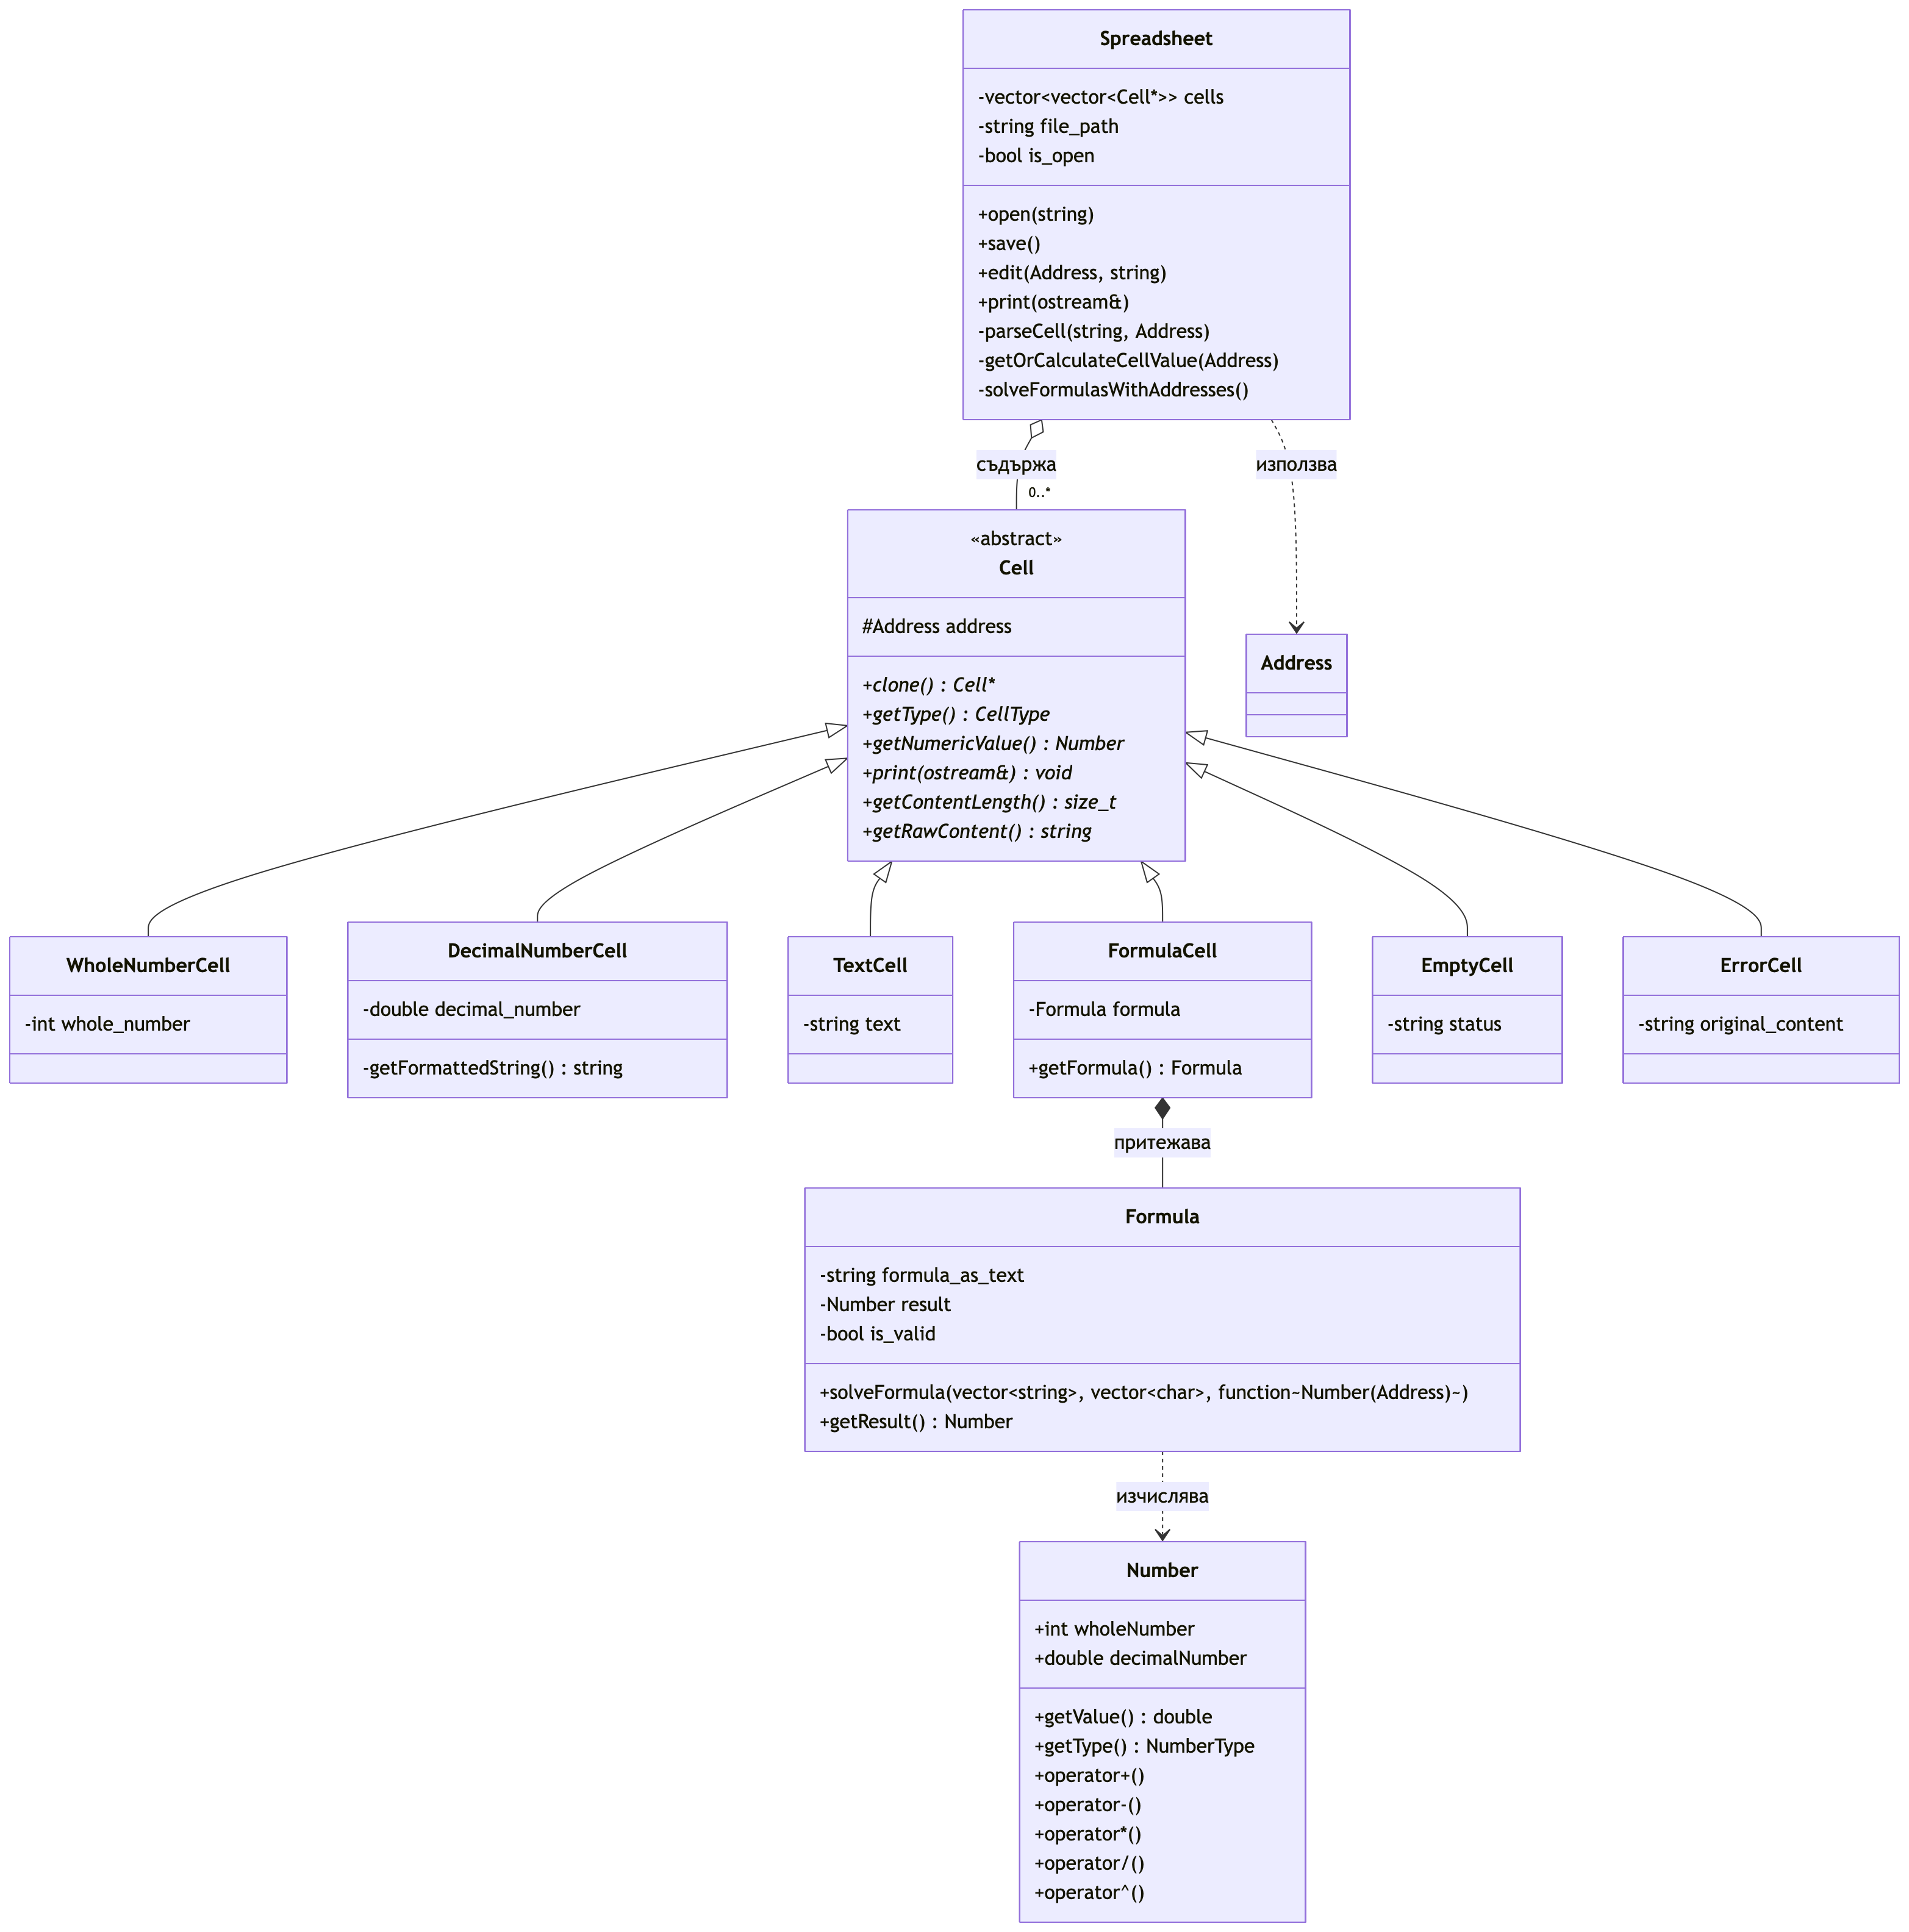
\includegraphics[width=0.9\textwidth]{images/class_diagram.png}
  \caption{Структурна диаграма на класовете}
  \label{fig:class_diagram}
\end{figure}

\subsection*{Поведенчески модел: Индиректно извличане на стойности}
Следната извадка от метода \texttt{getOrCalculateCellValue} демонстрира ключовия поведенчески модел – как \texttt{Spreadsheet} обработва формулите и им подава ламбда функция, улавяйки указателя \texttt{this}. Това позволява на обекта \texttt{Formula} да извлича стойности от други клетки в реално време. Преди извикването, клетката временно получава статус \texttt{"CALCULATING"}, за да се предотврати безкрайна рекурсия:

\begin{lstlisting}[language=C++]
std::vector<std::string> tokens;
std::vector<char> operators;

std::string formulaText = formula.getFormulaText();
tokenize(formulaText, tokens, operators);

// Временно заместване за защита от циклични препратки
delete cells[a.row - 1][a.col - 1];
cells[a.row - 1][a.col - 1] = new EmptyCell(a, "CALCULATING");

try
{
    // Подаване на ламбда функция, чрез която формулата
    // получава възможност индиректно и рекурсивно да
    // извлича непресметнати стойности
    formula.solveFormula(tokens, operators,
        [this](Address a) {
            return this->getOrCalculateCellValue(a);
        });

}
catch (const std::runtime_error &e)
{
    delete cells[a.row - 1][a.col - 1];
    cells[a.row - 1][a.col - 1] = new ErrorCell(a, formulaText);
    throw;
}
\end{lstlisting}